\documentclass[10pt]{article}
\usepackage{icmlko}

\icmlmeta{IP 파운데이션 월드모델}{337}{네 번째 목록}{위키 캐시에 894건이 있었는데 읽는 목록에 네 도메인이 없었다 --- 아이돌이 $+$0.074 를 그냥 갖고 있었다}

\begin{document}

\twocolumn[
\icmlheader

\begin{abstract}
노트 336이 ``목록이 둘이면 언젠가 갈라진다''를 남기고 \textbf{다른 축에도
갈라진 목록이 있나}를 갈래로 뒀다. 훑었다. \textbf{있다.}

\texttt{lab/wikiaxes.AXF} 가 여섯 도메인뿐이다(세계애니 · 만화 · 애니 ·
게임 · 모바일 · 웹툰). 그런데 \texttt{ingest/wiki\_views.SRC} 는 \textbf{열}
을 긁고, 캐시에는 \textbf{도서 212 · 펀딩 399 · 아이돌 78 · 시장팝업 205}
= 894건이 이미 있었다. \textbf{노트 178이 도서 · 펀딩을 쓰는 쪽에만
넣었고 읽는 쪽은 안 고쳐졌다.} 노트 336의 \texttt{trendaxes.FILE} 과 같은
자리 --- \textbf{네 번째다.}

넷을 넣으면 덮음이 \textbf{아이돌 82\% · 시장팝업 38\% · 도서 21\% ·
펀딩 0.5\%} 다. 짝지어(학습 재추출 열둘) 재면

\begin{center}\footnotesize
\begin{tabular}{lrrr}
\hline
도메인 & 덮음 & 짝지은 차 & 양수 \\
\hline
\textbf{아이돌} & \textbf{82\%} & \textbf{$+$0.0737} & \textbf{11/12} \\
시장팝업 & 38\% & $-$0.0237 & 6/12 \\
도서 & 21\% & $+$0.0074 & 8/12 \\
펀딩 & 0.5\% & $+$0.0050 & 9/12 \\
\hline
\textbf{판} & & \textbf{$+$0.0007} & 6/12 \\
\hline
\end{tabular}
\end{center}

\textbf{덮음이 높은 하나만 번다.} 노트 335가 ``열은 정보와 무관한 값이
있다''를 쟀는데, 여기서 그 값이 얼마나 되는지가 보인다 --- \textbf{덮음
38\% 와 21\% 는 그 값을 못 넘는다.}

\textbf{판은 안 움직인다}($+$0.0007 · 미결정 폭 안) \textbf{그리고 어느
도메인도 문턱 밖으로 안 내려간다.} 배포 규칙 ①②를 통과하고,
\textbf{점수로 고른 것이 아니라 목록이 틀려 있었다}(노트 82 · 90).
고쳤다.
\end{abstract}
]

\section{네 번째 목록}

\begin{center}\footnotesize
\begin{tabular}{lll}
\hline
층 & 어디 & 노트 \\
\hline
거르는 쪽 & \texttt{ingest/idol\_axes} & 326 \\
긁는 쪽 & \texttt{wiki\_views.idol\_items} & 332 \\
 & \texttt{idol\_album\_meta.run} & 333 \\
읽는 쪽(검색) & \texttt{trendaxes.FILE} & 336 \\
\textbf{읽는 쪽(위키)} & \texttt{wikiaxes.AXF} & \textbf{337} \\
\hline
\end{tabular}
\end{center}

\textbf{다섯 자리가 같은 모양이다} --- 한쪽만 고쳐졌고 다른 쪽은 그대로다.
그리고 \textbf{매번 조용했다}: 덮음 0\%는 ``자료가 없다''로 읽혔다.

\begin{figure*}[t]
\centering
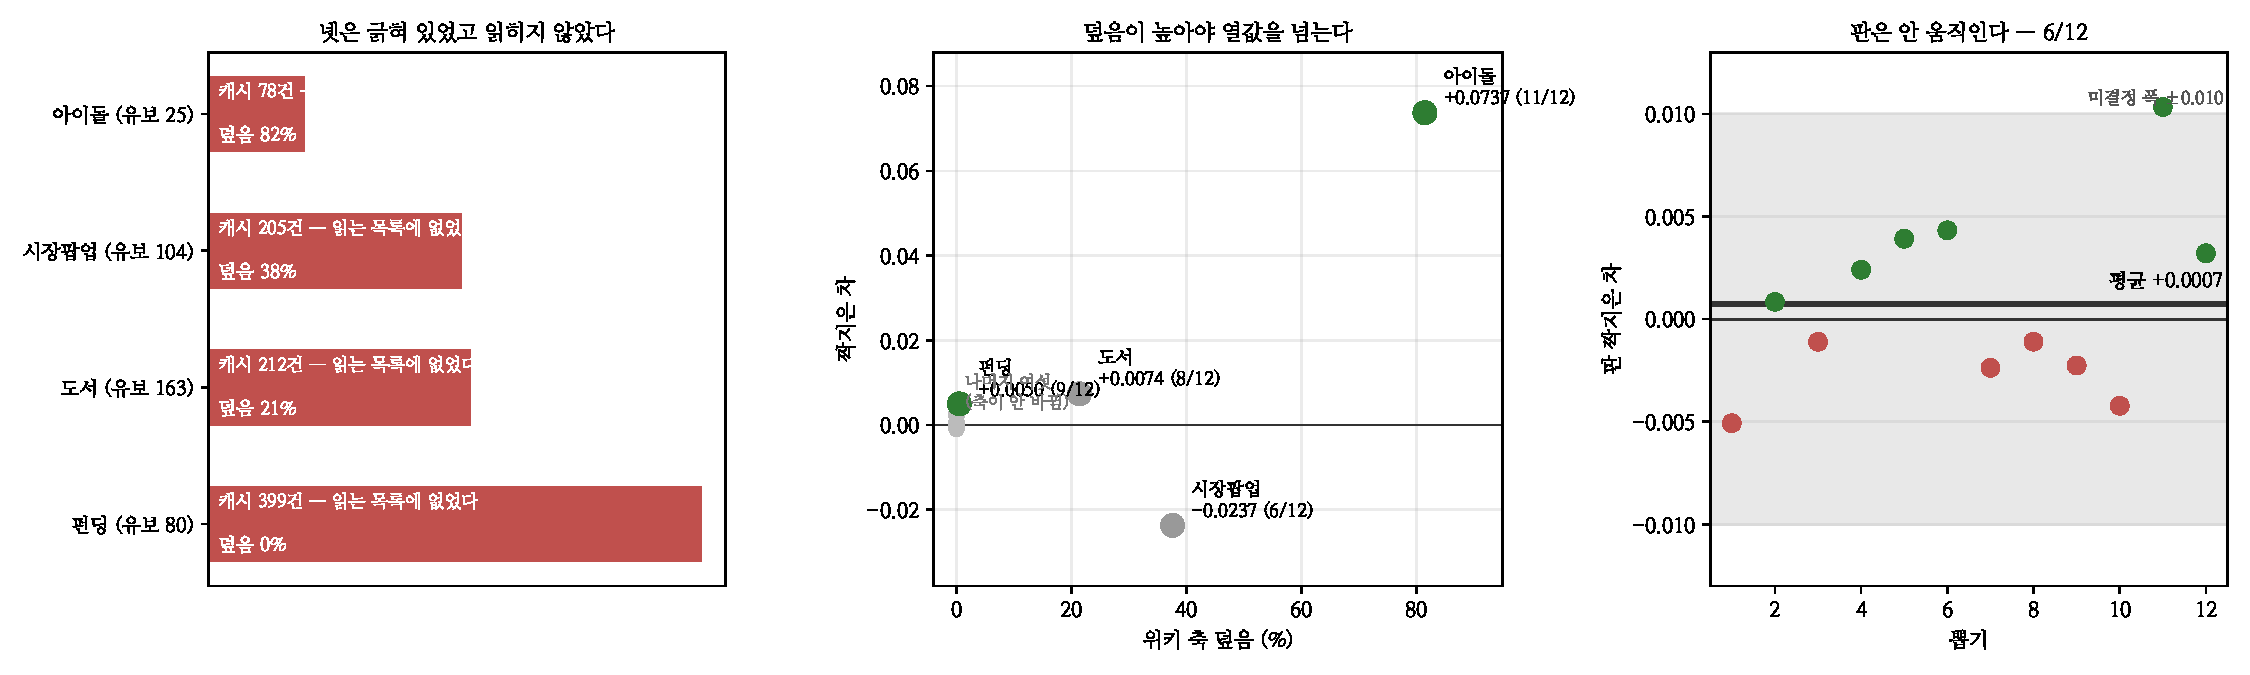
\includegraphics[width=\textwidth]{figs/fourth.pdf}
\caption{왼쪽 --- 캐시에 있었지만 안 읽힌 넷. 가운데 --- 덮음과 이득.
오른쪽 --- 판.}
\end{figure*}

\section{덮음이 열값을 넘어야 번다}

\begin{center}\small
\begin{tabular}{lrr}
\hline
 & 덮음 & 짝지은 차 \\
\hline
\textbf{아이돌} & 82\% & \textbf{$+$0.0737 (11/12)} \\
시장팝업 & 38\% & $-$0.0237 (6/12) \\
도서 & 21\% & $+$0.0074 (8/12) \\
펀딩 & 0.5\% & 축이 안 생긴다 \\
\hline
\end{tabular}
\end{center}

노트 335가 유보 25행에서 \textbf{정보 없는 열도 $-$0.05} 라고 쟀다.
여기 아이돌은 같은 25행인데 \textbf{$+$0.074} 다 --- 위키 축 넷(열 여덟)을
덮음 82\%로 붙였다. \textbf{같은 도메인 · 같은 열 수인데 부호가 반대다.}

\begin{center}\footnotesize
\begin{tabular}{lrrr}
\hline
아이돌에 무엇을 붙였나 & 덮음 & 열 & 차 \\
\hline
앨범 축 둘(노트 335) & 84\% & 4 & $-$0.05 \\
\textbf{위키 축 넷}(오늘) & 82\% & 8 & \textbf{$+$0.07} \\
\hline
\end{tabular}
\end{center}

\textbf{덮음도 열 수도 답이 아니다.} 다른 것은 \emph{이미 몇 열이 있었나}다
--- 앨범 축은 위키 · 검색을 이미 붙인 판(축 스물셋)에 더한 것이고, 위키는
공유 다섯만 있던 판에 더한 것이다. \textbf{열의 한계값은 이미 있는 열
수에 달렸다}는 것이 지금 서 있는 설명이고, 아직 안 쟀다.

\section{판}

\begin{center}\small
\begin{tabular}{lr}
\hline
판 짝지은 차 & $+$0.0007 (SD 0.0043 · 6/12) \\
제일 나쁜 도메인 & 시장팝업 $-$0.0237 (짝SE 0.04) \\
\hline
배포 규칙 ①② & \textbf{통과} \\
\hline
\end{tabular}
\end{center}

\textbf{자료 결정이다}(노트 82 · 90) --- 목록이 틀렸으니 고쳤다. 점수를
보고 넷 중 하나를 고르지 않는다.

\section{남은 것}
\begin{center}\footnotesize
\begin{tabular}{ll}
\hline
갈래 & 왜 \\
\hline
\textbf{열의 한계값을 재라} & 축 다섯일 때와 스물셋일 때 \\
목록 감사를 도구로 & 다섯 번 손으로 찾았다 \\
시장팝업 $-$0.024 & 덮음 38\%가 모자란가 \\
펀딩 위키 0.5\% & 400건 긁어 둘 --- 제목이 문제 \\
\hline
\end{tabular}
\end{center}

\paragraph{규약} \textbf{긁어 놓고 안 읽는 자료가 있다.} 이 실험실은
``무엇을 더 긁을까''를 여러 번 물었는데(노트 149 · 178 · 332 · 333),
\textbf{``이미 긁은 것을 다 읽고 있나''는 한 번도 안 물었다.} 오늘 세어 보니
위키 캐시 894건이 읽히지 않고 있었고 그중 아이돌 78건이 $+$0.074 짜리였다.
\textbf{수집은 비싸고 목록 대조는 공짜다} --- 다음부터 수집 과제를 세우기
전에 목록부터 맞춘다.

\end{document}
